%
% include the class file for USI-INF Technical Reports
%
\documentclass{usiinftr}

%
% if you want to create a cover page only (e.g. to put it in front
% of a WORD document or the like), use the "coverpage" option
%
%\documentclass[coverpage]{usiinftr}

%%%%%%%%%%%%%%%%%%%%%%%%%%%%%%%%%%%%%%%%%%%%%%%%%%%%%%%%%%%%%%%%%%%%

\begin{document}

%
% put the title of the Technical Report here
%
\title{A High Performance Video Segmentation Framework}

%
% put the author names here; use the second argument as a
% reference to the list of affiliations
%
\author{Liudmila Karagyaur}{1}
\author{Lorenzo Ferri}{1}
\author{Vanessa Braglia}{1}

%
% put the affiliations of the authors here
% NOTE: use the macro "\USIINF" for our Faculty of Informatics
%
\affiliation{1}{\USIINF}

%
% put the number of your Technical Report here; in order to determine
% the number, take the number of the most recent USI INF Technical Report
% (on top of the list at http://www.inf.usi.ch/techreports/) and increment
% it by one; the format is "[year]-[number]"
%
\TRnumber{2010-4}

%
% by default, the current month and year are used as the publication date
% of your Technical Report; if you want to change this, then you can do it here, e.g.
%
%\date{February~\the\year}
%\date{August 2011}

%
% the rest is as usual
%

%%%%%%%%%%%%%%%%%%%%%%%%%%%%%%%%%%%%%%%%%%%%%%%%%%%%%%%%%%%%%%%%%%%%

\maketitle

\begin{abstract}
Edge detection is a ubiquitous technique in scientific computing. It is widely utilised in content based video retrieval for the search of digital information in large datasets, and plays also a critical role in the development of self-driving vehicles that need to perform real-time feature detection.
We present a high performance video segmentation framework that is able to find the main features of a video, and to follow their trajectories. Initially, we evaluate the performance and solution quality of k-means clustering algorithms, in order to ensure that it is a suitable choice for the application at hand. Subsequently, a convolutional neural network is trained to label the obtained clusters, thus enabling the extraction of the main features of the video. The process is executed in parallel for each frame of the video, in order to reduce the overall run time of the routine.
\end{abstract}

\section{Introduction}
Nowadays edge detection techniques have several applications. For example, a content based video retrieval is widely required for searching digital information in large databases, in order to improve text based retrieval systems \cite{1}. It also has an important role in the development of self-driving vehicles, that need to perform a real-time feature detection \cite{2}, and in medical field, in the analysis of digital images of pathological conditions, such as tumors \cite{3}. \\
The goal of this project is to find the main features of a video and to be able to follow their trajectories. In particular, we will analyse single video frames using edge detection, which is an image segmentation technique. \\
There exists a great variety of clustering algorithms that perform efficient image segmentation, which is a fundamental step in feature extraction. The first step consists in detecting a clustering algorithm that suits better the problem at hand. 
However, before applying clustering algorithm to the frames it is convenient to get rid of the possible influence of the secondary objects. For this purpose the background will be set to black on each frame before proceeding with the analysis. \\
Once the clusters are well defined, a classifier will label the objects of our interest and finally the video will be reconstructed with only its critical features. At the end, the edge detection will be executed in parallel on each frame of the video, in order to improve the performance. \\
The paper will be organized as follows. In section 2 will be presented the algorithms and the techniques used to accomplish the project, such as k-means and connected components clustering, convolutional neural network and multiprocessor parallelization. In section 3, our application will be introduced. The procedures described will be applied to a pool game video and the results will be visually presented  after each step. 

\section{Algorithms and Techniques}
The project is organized in 4 main steps. The first task to be completed is the application of the k-means clustering algorithm to the video, previously subdivided in frames. The goal is to be able to identify the main features among other secondary objects and obtain isolated clusters for each of them. In order to facilitate this task the background of each frame is set to black before applying the clustering algorithm. To obtain the desired result we have applied the k-means clustering two times: the first time it is applied on the frame to detect the main features and the second time on each resulting cluster generated in the previous step. The purpose of this second call is to remove the noise from those clusters that contain the main features of the frame. \\
Now we have to distinguish between the clusters that contain the main items of the video and those that consist of noisy components. In order to do that we are going to use a convolutional neural network that is going to label all the generated clusters, identifying the ones that will be processed in the later stages. \\
Each cluster classified as main component of the frame is then exposed to a an algorithm that identifies all the connected components. The goal we want to reach is the partition of the cluster in its individual items.  \\
The final step consists in reducing the overall run time of the routine and this will be done by executing the whole process in parallel for a suitable number of frames, depending on the number of processors available in the machine.
\subsection{\textit{k}-means clustering algorithm} 
The k-means algorithm is the simplest and most popular clustering algorithm. Its ultimate goal is to partition $n$ initial datapoints into $k$ clusters. It requires that the user provides the number $k$ of clusters that have to be found. The algorithms uses an iterative approach: starting from an initial set of random centroids, at each iteration it generates the clusters by minimizing the Euclidean distance $D$ between each point $x_i$  and  the centroids $c_j$:  
$$\arg \min\limits_{j}D(x_i, c_j)\;\;\;\; j = 1, \dots, k$$
Then, for each cluster $C_j$ a new centroid $c_j$ is computed as the mean of all $n_j$ points $x_i$ assigned to the cluster in the previous step: 
$$c_j = \frac{1}{n_j} \sum_{x_i \in C_j} x_i$$
Convergence is achieved when points are no longer interchanged between the clusters.
In the particular case of this application the distance between the pixels is computed considering their colour in RGB format. This means that the data point $x_i$ will be represented by a three-dimensional array, which elements will correspond to the R, G, and B components of the colour. \\
A visual representation of the \textit{k}-means algorithm can be observed in Figure \ref{fig:1}
\begin{figure}[h]
	\centering
	\includegraphics[width=0.6\linewidth]{./img/k_means}
	\caption{\textit{k}-means clustering algorithm}
	\label{fig:1}
\end{figure}


\subsection{Connected Components}
Connected components is a valid alternative to more common clustering algorithms like k-means or Spectral clustering. 
Connected components is an algorithm that applies concepts of the graph theory in order to identify those sets of nodes that are considered similar based on a given heuristic. In particular, two nodes are considered part of the same connected component if there is a path between them. \\
Identifying connected components could be a very useful tool if we want to isolate clusters in a set of items. 
The application of this algorithm on images will consider each pixel as one node of the graph. The metric used to evaluate the connection between two nodes is based on the colour of the pixels. A weighted alternative of the algorithm can also be considered. It recognizes two pixels in the same connected component if their distance in terms of colour is above a certain threshold.

\begin{figure}[h]
	\centering
	\includegraphics[width=0.4\linewidth]{img/connected_components}
	\caption{A visual representation of a graph with 3 connected components}
	\label{fig:2}
\end{figure}


\subsection{Convolutional Neural Network}
\textbf{LORE LAVORA}



\subsection{Multiprocessor parallelization}
Multiprocessors refers to the use of two or more CPUs (central processing units) contained in a single computer system that supports the execution of threads collaborating on a single task. The coordination and the usage of the single processors is controlled by the same operating system and all the processors share the same main memory by means of a shared address space.  \\
The usage of multiple processors instead of one presents several advantages. One of the most important ones is the increasing of the  throughput, which means that more work can be executed and completed in a unit time. However, an important drawback could be the cost of the communication among different processors. For this reason the parallelization of a program with multiprocessing is particularly convenient if the tasks are independent of each other.

\begin{figure}[h]
	\centering
	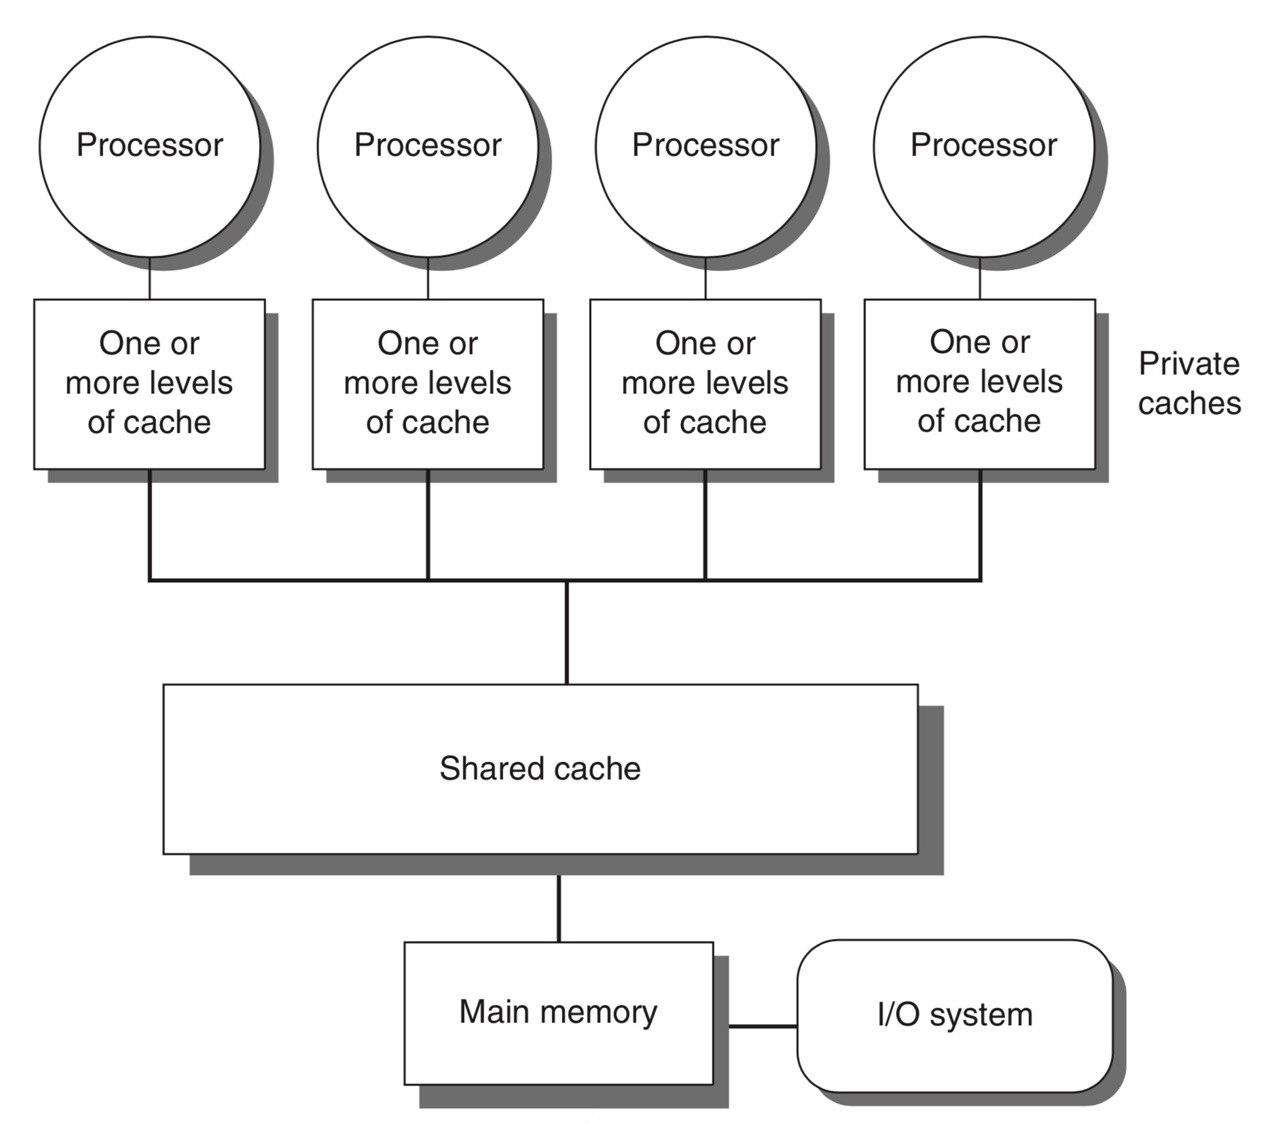
\includegraphics[width=0.5\linewidth]{img/multiprocessing}
	\caption{Structure of a centralized shared-memory multiprocessor}
	\label{fig:3}
\end{figure}



\section{Numerical Results}
%The output generated by this algorithm is a partition of each cluster containing the main features, in its individual units.


\section{Conclusions}

\bibliographystyle{unsrt}  
%\bibliography{references}  %%% Remove comment to use the external .bib file (using bibtex).
%%% and comment out the ``thebibliography'' section.


%%% Comment out this section when you \bibliography{references} is enabled.
\begin{thebibliography}{1}
	
	
	\bibitem {1}
	B.V. Patel and B.B. Meshram,
	\textit{Content Based Retrieval Systems},
	International Journal of UbiComp (IJU), Vol.3, No.2, 
	April 2012
	
	\bibitem {2} 
	H. Cho, Y. Seo, B. V. K. V. Kumar and R. R. Rajkumar, 
	\textit{A multi-sensor fusion system for moving object detection and tracking in urban driving environments}, 
	IEEE International Conference on Robotics and Automation (ICRA), 
	2014
	
	\bibitem {3} 
	Ed-Edily Mohd,  Azhari,Muhd. Mudzakkir Mohd. Hatta, Zaw Zaw Htike,  Shoon Lei Win, 
	\textit{Tumor detection in medical imaging: a survey }, 
	International Journal of Advanced Information Technology (IJAIT) Vol. 4, No. 1, 
	February 2014
	
	
\end{thebibliography}


%%%%%%%%%%%%%%%%%%%%%%%%%%%%%%%%%%%%%%%%%%%%%%%%%%%%%%%%%%%%%%%%%%%%

\end{document}
